\section{Introduction}

Large Language Models (LLMs), despite their impressive performance across various natural language understanding tasks, exhibit significant limitations when applied to enterprise applications in the wild.
Primarily, these models may hallucinate—generating plausible-sounding but factually incorrect content—when their parametric knowledge does not align with specific enterprise data~\cite{maynez2020faithfulness,semnani2023wikichat,feng2024cmdbench}
. An LLM's parametric knowledge depends on its pre-training corpus and can also be influenced by the chosen training strategy and model architecture. This gap is especially problematic since enterprise applications frequently use private, on-premises data, which may differ substantially from the domains in LLMs' pre-training corpora.
Such domain misalignment can lead to severe inaccuracies, where the LLMs produce unreliable or misleading information.
%
In addition, enterprises often require consistency and reliability in their outputs. However, LLMs can be sensitive to prompt wording \cite{sclar2024quantifying}, producing inconsistent results even with minor phrasing changes, which undermines their reliability in high-stakes enterprise tasks.


Another key challenge for LLMs in enterprise settings is their limited capacity for complex reasoning. Many tasks in this domain require multi-step reasoning, deep contextual understanding, and coherent integration across different data sources, models, and pipelines. LLMs are not inherently designed to manage such complexities without extensive, task-specific adaptation and external grounding. These limitations hinder adopting LLMs in enterprise fields where accuracy, consistency, and reasoning depth are critical, such as healthcare, legal, HR, and data-driven decision-making applications.



%
Several approaches can help mitigate these limitations, including controlled generation, fact-checking, and post-processing. Controlled generation seeks to constrain the outputs of LLMs by guiding the model toward more reliable responses through techniques such as prompt engineering~\cite{brown2020language,wei2022chain,sahoo2024systematic}, fine-tuning~\cite{houlsby2019parameter,qin2023towards}, and reinforcement learning from human feedback~\cite{ouyang2022training}.
Fact-checking~\cite{thorne-etal-2018-fever,aly2021feverous} involves verifying generated content against highly credible sources to ensure accuracy, with any identified inaccuracies filtered out or corrected during post-processing. 
Although these techniques offer improvements, they may still struggle with domain-specific challenges and rapidly evolving knowledge.
\begin{figure}[t!] 
  %\vspace{-10pt}
  \centering
  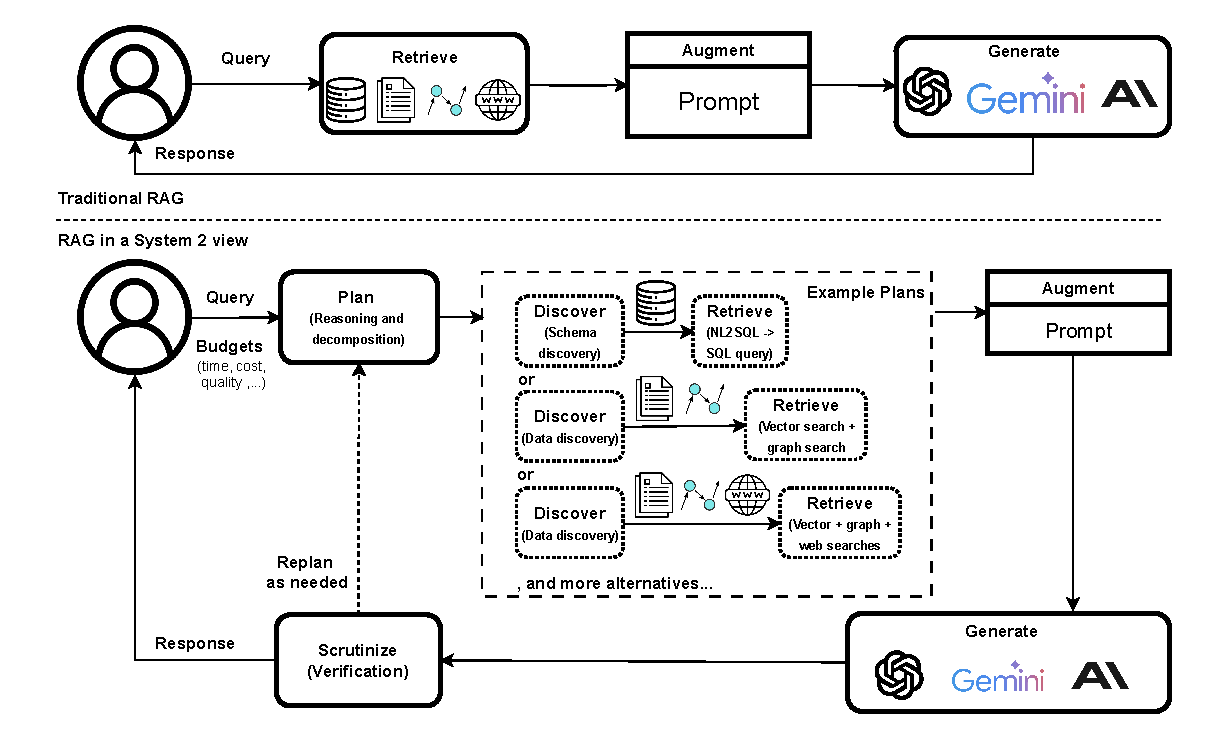
\includegraphics[width=\linewidth]{submissions/Estevam2024/figures/sys-rag2.pdf}
  \caption{Compared to the traditional RAG setup (above), where a fixed Retrieval-Augmentation-Generation workflow is executed, a System 2 approach (below) involves more deliberate reasoning and action based on critical analysis. For instance, given the same user query, the system must first plan by analyzing the task and may decide to decompose it into smaller components, such as data discovery, natural language-to-query translation, and actual query execution. During the planning phase, constraints or budgets related to factors like time, cost, or quality, along with the nature of the multimodal data sources, may influence the direction of the workflow. After the generation step, a verification process is typically required to evaluate the outcome, which may lead to revisions in subsequent iterations.}
  \label{fig:sys-rag2} 
\end{figure}
Among the various approaches, augmenting LLMs with external information sources has emerged as one of the most widely adopted solutions for enhancing accuracy and robustness. 
This strategy enables LLMs to access up-to-date, domain-specific knowledge, making them more adaptable to new fields or emerging topics. 
Techniques like retrieval-augmented generation (RAG)~\cite{lewis2020retrieval} integrate external databases or knowledge graphs to ground the model's outputs in verifiable information. 
By incorporating external data, such as multi-modal documents or enterprise-specific datasets, LLMs can produce more accurate and contextually relevant responses, thereby reducing the likelihood of hallucinations and making them more suitable for critical applications. However, simply using RAG approaches is not necessarily yet the definitive solution. Challenges remain, such as ensuring the quality and reliability of the retrieved information, handling ambiguous or conflicting data, and seamlessly integrating retrieval with generation to maintain coherent and contextually appropriate responses. Consequently, there is still considerable room for improvement in creating more robust and reliable AI systems.



As already shown in the literature, the idea of \emph{System 1} and \emph{System 2} \cite{kahneman_thinking_2012},  can be helpful to contextualize the current capabilities and limitations of LLMs \cite{bengio2019system}. In cognitive sciences, \emph{System 1} refers to fast, intuitive, and automatic thinking. This type of system can be characterized by fast thinking or quick judgments and decisions that rely on heuristics and subconscious processing. System 1 is highly efficient for everyday tasks that require intuitive, fast, unconscious, and immediate responses.
System 2, however, is associated with slow, deliberate, and analytical thinking. It is more helpful and used for complex problem-solving, critical analysis, and tasks that require conscious, sequential, algorithmic planning and reasoning. System 2 is more resource-intensive and slower but more reliable for tasks requiring careful consideration. 

In this System~1/System~2 context, we argue that even though RAG approaches have strong potential to contribute to reducing limitations of current LLMs (by playing a role more closely related to System 2), most current RAG approaches only weakly resemble System 2 thinking. The retrieval and generation steps are often designed to be fast and instantaneous, aligning with System 1 thinking, rather than slow and logical as in System 2, which presents challenges on both the data and model sides. For example, research \cite{maekawa-etal-2024-retrieval,ding2024retrieve} has shown that augmenting LLMs with retrieval without rigorously assessing necessity may adversely impact overall performance. 



Therefore, as illustrated in Figure~\ref{fig:sys-rag2}, we advocate for a shift from traditional single-model architectures to compound AI systems within a System 2 framework to enhance RAG, particularly in complex enterprise applications. Compound systems enable a collaborative approach to problem-solving by distributing specialized tasks across distinct agents, each optimized for specific functions, improving both retrieval and generation performance in challenging real-world settings.

On the retrieval side, enterprise applications often involve complex, multi-step, and sometimes ambiguous tasks that require deeper reasoning and structured workflows. A compound system can enhance this by assigning specialized agents to handle diverse aspects of data, such as heterogeneous formats (e.g., text, tables, graphs, parametric information) and noisy or incomplete data sources. This allows for agents skilled in reconciliation and semantic querying to refine the retrieval process through iterative, logic-driven interaction, improving both precision and relevance of context.

On the generation side, challenges like hallucination, fact verification, and adherence to context remain key obstacles. In a compound system setup, individual agents can be tasked with verifying facts, maintaining context alignment, and evaluating outputs for accuracy before finalizing responses. This division of labor can be exploited towards reducing hallucinations and enhancing reliability by enabling dynamic inter-agent evaluation, where each agent iteratively cross-checks and validates the others' outputs \cite{zhang2021survey,carlson2010toward}. For example, in domain-specific conversational AI, particularly in regulated industries, compound AI systems offer a pathway to safer, more reliable, and robust deployments by integrating domain expertise, context sensitivity, and rigorous validation at each step. 


The paper is organized as follows. First, in \cref{sec:background}, we provide a brief overview of traditional RAG models and highlight their limitations, especially in real-world, domain-specific applications. We then motivate more concretely the need for a System 2 RAG approach, in section 3. In \cref{sec:sys2}, several approaches to enhance RAG adaptability to System 2 thinking are discussed. Finally, we present our vision for future research in \cref{sec:future}, exploring the potential of compound AI systems as System 2 solutions to RAG.

